\documentclass{article}

\usepackage[utf8]{inputenc}
\usepackage{hyperref}
\usepackage [english]{babel}
\usepackage [autostyle, english = american]{csquotes}
\MakeOuterQuote{"}
\hypersetup{
    colorlinks=true,
    linkcolor=blue,
    filecolor=magenta,      
    urlcolor=cyan,
}
\usepackage{xcolor}
\usepackage{listings}
\lstdefinestyle{BashInputStyle}{
  language=bash,
  basicstyle=\small\sffamily,
  numbers=left,
  numberstyle=\tiny,
  numbersep=3pt,
  frame=tb,
  columns=fullflexible,
  backgroundcolor=\color{yellow!15},
  linewidth=0.9\linewidth,
  xleftmargin=0.1\linewidth
}
\usepackage{graphics}
\usepackage{graphicx}
\usepackage{pdflscape}
\usepackage{afterpage}
\usepackage{capt-of}
\usepackage{fontspec,fontawesome}
\graphicspath{ {images/} }

\title{RasPi-Fog : End User Tutorial}

\author{Shreshth Tuli$^{1}$}
\date{June 2018}


\begin{document}
\maketitle

\section{Introduction}
This tutorial or step-by-step guide shows you how to setup your own Fog-Computing Environment using Raspberry Pi's or similar edge node devices used for IoT applications. This specific tutorial is to setup a "Sleep Apnea Analyzer" which provides a user with Sleep Apnea disease severity and other parameters for in depth analysis.\\ \\
Using Apache server and HTTP REST APIs you will be able to setup communication between Fog devices having a Master/Slave architecture. A "Master" is the Fog node that distributes work between the "Slave" or "Worker" nodes. A Master can itself also act as a Worker. 

\section{Material Required}
For the Fog-Computing setup the following would be required:
\begin{enumerate}
\item 2 or more Raspberry Pi's : \href{https://www.amazon.com/Raspberry-Pi-RASPBERRYPI3-MODB-1GB-Model-Motherboard/dp/B01CD5VC92/ref=sr_1_3?s=pc&ie=UTF8&qid=1528948400&sr=1-3&keywords=raspberry+pi+3}{Amazon Link}
\item HDMI cable : \href{https://www.amazon.com/AmazonBasics-High-Speed-HDMI-Cable-1-Pack/dp/B014I8SSD0/ref=sr_1_1_acs_sk_pb_1_sl_1?ie=UTF8&qid=1528948612&sr=8-1-acs&keywords=HDMI+Cable}{Amazon Link}
\item Keyboard-Mouse : \href{https://www.amazon.com/AmazonBasics-Wired-Keyboard-Mouse-Bundle/dp/B00B7GV802/ref=sr_1_1_sspa?s=electronics&ie=UTF8&qid=1528948656&sr=1-1-spons&keywords=keyboard+mouse&psc=1}{Amazon Link}
\item Micro SD cards (Atleast 8 GB) : \href{https://www.amazon.com/dp/B073JYVKNX/ref=sxts_k2p-hero-vn_bs_1?pf_rd_m=ATVPDKIKX0DER&pf_rd_p=3338417525430323799&pd_rd_wg=uUtqX&pf_rd_r=J02KSGBGGGV7S9B4CYZW&pf_rd_s=desktop-sx-top-slot&pf_rd_t=301&pd_rd_i=B073JYVKNX&pd_rd_w=4K3bM&pf_rd_i=micro+sd+card&pd_rd_r=8057615f-9cb8-4c23-ace6-39218b385876&ie=UTF8&qid=1528948722&sr=1}{Amazon Link}
\item Micro SD to SD adapter : \href{https://www.amazon.com/SanDisk-microSD-Memory-Adapter-MICROSD-ADAPTER/dp/B0047WZOOO/ref=sr_1_3?s=electronics&ie=UTF8&qid=1528949416&sr=1-3&keywords=micro+sd+to+sd+adapter}{Amazon Link}
\item Monitor with HDMI input
\item USB Pendrive (Atleast 1 GB)
\item 5V - 2A power supplys with Micro USB output (Either of the two options) 
\begin{itemize}
\item Power Adapter : \href{https://www.amazon.com/dp/B073JYVKNX/ref=sxts_k2p-hero-vn_bs_1?pf_rd_m=ATVPDKIKX0DER&pf_rd_p=3338417525430323799&pd_rd_wg=uUtqX&pf_rd_r=J02KSGBGGGV7S9B4CYZW&pf_rd_s=desktop-sx-top-slot&pf_rd_t=301&pd_rd_i=B073JYVKNX&pd_rd_w=4K3bM&pf_rd_i=micro+sd+card&pd_rd_r=8057615f-9cb8-4c23-ace6-39218b385876&ie=UTF8&qid=1528948722&sr=1}{Amazon Link}
\item Power Bank : \href{https://www.amazon.com/KMASHI-15000mAh-External-Portable-Powerful/dp/B00JP8MZGK/ref=sr_1_3?s=electronics&ie=UTF8&qid=1528949090&sr=1-3&keywords=5v+2a+power+bank}{Amazon Link}
\end{itemize}
\item A PC with SD Card, USB slots and WiFi
\end{enumerate}

\section{Circuit}
Connect the devices as per following steps:
\begin{enumerate}
\item Connect the Raspberry-Pi with keyboard and mouse.
\item Connect the Monitor to the Pi using HDMI Cable.
\item Power on the Monitor
\item Provide power to the Pi through adapter or power bank. 
\end{enumerate}
The final circuit is shown below. 
\begin{figure}[h]
\centering % Center table
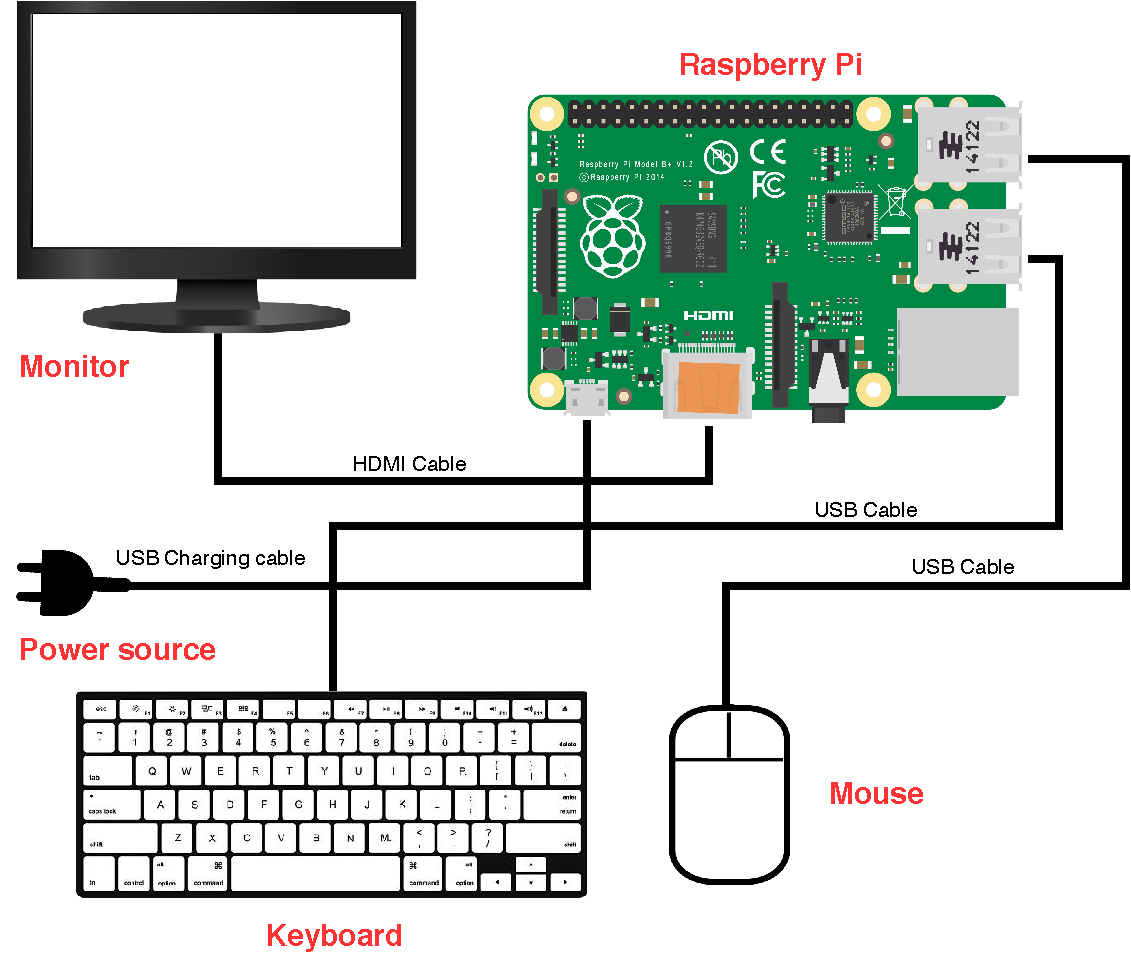
\includegraphics[width=13cm]{raspi-fog-circuit}
\captionof{figure}{Circuit Diagram}
\end{figure}

\newpage

\section{Install OS}
On PC follow the following steps:
\begin{enumerate}
\item Download the Raspberry Pi OS image : "Raspbian Stretch Desktop" from this \href{https://downloads.raspberrypi.org/raspbian_latest}{link}
\item Download and Install Disk Image flashing software like "Etcher" from \href{https://etcher.io/}{here}.
\item Insert the Micro SD card inside the Micro SD to SD adapter and then insert the adapter to the SD Card slot in the PC
\item Run "Etcher" Software. Select the downloaded Raspbian image file, the SD Card drive and click on "Flash".
\item When flashing and validation is over, eject the SD card adapter. 
\item Repeat steps 3 to 5 for other Micro SD cards
\item Remove power cable from Raspberry Pi and insert the Micro SD Card. Re-insert the power cable into the Pi.
\end{enumerate}

The Raspberry Pi would now boot up and is ready to install the required softwares for the Fog-Computing environment.

\section{Installing Raspi-Fog : Worker}

\subsection{Raspberry Pi or other Linux machines}
Open Terminal by pressing simultaneously : Ctrl-Alt-T and type in the following commands: 
\subsubsection{Install Java}
\begin{lstlisting}[style=BashInputStyle]
    sudo apt-get update
    sudo apt-get upgrade
    sudo apt-get install oracle-java8-jdk -y
    sudo apt-get install ant git vim -y
\end{lstlisting}
\subsubsection{Install Apache, PHP and MySQL}
\begin{lstlisting}[style=BashInputStyle]
    sudo apt-get install apache2 -y
    sudo vim /etc/apache2/apache2.conf
\end{lstlisting}
Now on the bottom of the file type "i" to append document and add the following line:
\begin{lstlisting}[style=BashInputStyle]
    ServerName 127.0.0.1
\end{lstlisting}
To test Apache run:
\begin{lstlisting}[style=BashInputStyle]
    sudo apache2ctl configtest
\end{lstlisting}
The output of this command should be : "Syntax OK". If yes, then Apache is installed and configured properly. \\Now install PHP and MySQL using:
\begin{lstlisting}[style=BashInputStyle]
    sudo apt-get install php libapache2-mod-php php-mcrypt php-mysql -y
    sudo service apache2 restart
    sudo apt-get install mysql-server -y
    sudo mysql_secure_installation
\end{lstlisting}
When asked for password, enter "raspberry". For all other questions except the last question answer "n", and for last "y".\\
Now, configure MySQL and add database named "data" using:
\begin{lstlisting}[style=BashInputStyle]
    sudo mysql -u root -p
    CREATE DATABASE data;
    show databases;
    GRANT ALL PRIVILEGES ON data.* TO 'root'@'localhost' IDENTIFIED BY 'raspberry';
    FLUSH PRIVILEGES;
    exit;
\end{lstlisting}
Install PHPMyAdmin using:
\begin{lstlisting}[style=BashInputStyle]
    sudo apt-get install phpmyadmin -y
\end{lstlisting}
When prompted to choose server : select "Apache2". In the Configure PHPMyAdmin, select "No".\\ Now add PHPMyAdmin configuration to Apache2 using:
\begin{lstlisting}[style=BashInputStyle]
    sudo vim /etc/apache2/apache2.conf
\end{lstlisting}
In the end of file, select "i" to insert and add the following line:
\begin{lstlisting}[style=BashInputStyle]
    Include /etc/phpmyadmin/apache.conf
\end{lstlisting}
Restart apache service using:
\begin{lstlisting}[style=BashInputStyle]
    sudo service apache2 restart
\end{lstlisting}
Now, go to the html folder and add "HealthKeeper" scripts using following commands:
\begin{lstlisting}[style=BashInputStyle]
    cd /var/www/html/
    sudo mkdir HealthKeeper/
    sudo chmod -R 777 HealthKeeper/
\end{lstlisting}
Download "HealthKeeper" data from this \href{https://drive.google.com/open?id=1DZWaJHHNMrJFnsCfxoWSIpfDhK7n-qHH}{link} and transfer files in the "Worker" folder to the, just created, HealthKeeper folder. in the \textit{/var/www/html/} path.\\
On terminal run the following commands to run the Analyzer:
\begin{lstlisting}[style=BashInputStyle]
    cd /var/www/html/HealthKeeper
    sudo chmod 777 *
    javac ./analyzer.java
    java analyzer
\end{lstlisting}
In another tab of terminal run:
\begin{lstlisting}[style=BashInputStyle]
    hostname -I
\end{lstlisting}
It will show the IPv4 address of the machine. Note it for future use.

\subsection{Windows Machines}
Download XAMPP from the following \href{https://www.apachefriends.org/xampp-files/7.2.6/xampp-win32-7.2.6-0-VC15-installer.exe}{link} and Install XAMPP. Run XAMPP and start Apache and MySQL service.\\ \\
Go to \textit{C:/xampp/htdocs/} and create folder named "HealthKeeper". Download "HealthKeeper" data from this \href{https://drive.google.com/open?id=1DZWaJHHNMrJFnsCfxoWSIpfDhK7n-qHH}{link} and transfer files in the "Worker" folder to the HealthKeeper folder.\\ \\
Go to the folder \textit{C:/xampp/htdoxs/HealthKeeper/} and open terminal. Run the following commands to run analyzer:
\begin{lstlisting}[style=BashInputStyle]
    javac ./analyzer.java
    java analyzer
\end{lstlisting}
Press \faWindows \ + R, type "cmd" and then press "Enter". On the command prompt type "ipconfig" and note the IPv4 address for future use.

\section{Installing Raspi-Fog : Master}

For Linux and Windows Machines follow the steps for Worker Installation, but instead of copying the Worker folder files, copy the Master and Worker folder inside /HealthKeeper/RPi/ folder.\\ \\
Go to the folder \textit{C:/xampp/htdoxs/HealthKeeper/RPi/Worker/} and open terminal. Run the following commands to run analyzer:
\begin{lstlisting}[style=BashInputStyle]
    javac ./analyzer.java
    java analyzer
\end{lstlisting}
Press \faWindows \ + R, type "cmd" and then press "Enter". On the command prompt type "ipconfig" and note the IPv4 address for future use as the Master IP Address.

\section{Configuring Raspi-Fog}

On the master server, open browser and go to:
\begin{lstlisting}[style=BashInputStyle]
    http://localhost/phpmyadmin/
\end{lstlisting}
Follow the following steps to configure database:
\begin{enumerate}
\item Create new database by clicking "New" in the left column. Enter name = "users" and click "create".
\item Add a table in this database named "registrations" and having 3 columns.
\item Type the column names as "ID", "username" and "password". Keep "ID" column as primary key and of type INT. Keep others as VARCHAR. Click on "Save" to create table.
\item On the top tab, click on "Insert" to insert an entry. Type in 1 in ID, and "admin" in username and password.
\end{enumerate}

\subsection{Configuring Worker}
Open browser and go to:
\begin{lstlisting}[style=BashInputStyle]
    http://localhost/HealthKeeper/manager.php
\end{lstlisting}
Enter Master IP address as noted earlier.

\subsection{Configuring Master}
Open browser and go to:
\begin{lstlisting}[style=BashInputStyle]
    http://localhost/HealthKeeper/RPi/Master/manager.php
\end{lstlisting}
Add the IP addresses of the worker nodes noted earlier. Choose the "Enable Master as Worker" as per requirement.
\\Then go to:
\begin{lstlisting}[style=BashInputStyle]
    http://localhost/HealthKeeper/RPi/Master/
\end{lstlisting}
Login with username : "admin" and password : "admin". Enter data for analysis and press "Enter". Then click "Analyze" to get results.


\end{document}
